\documentclass[10pt,twocolumn,letterpaper]{article}

\usepackage{cvpr}
\usepackage{times}
\usepackage{epsfig}
\usepackage{graphicx}
\usepackage{amsmath}
\usepackage{amssymb}
\usepackage{float}
\usepackage{subfig}
\usepackage{algorithm2e}
\usepackage{setspace}
\usepackage[breaklinks=true,bookmarks=false]{hyperref}
\usepackage[capitalize]{cleveref}

\renewcommand\ttdefault{cmtt}

\cvprfinalcopy

\def\httilde{\mbox{\tt\raisebox{-.5ex}{\symbol{126}}}}

\setcounter{page}{1}
\begin{document}

\title{AlphaGoStop: Applying Deep Reinforcement Learning
to Go-Stop}

\author{20170058\quad Keonwoo Kim\\\normalsize\texttt{keonwoo@kaist.ac.kr / }\url{https://github.com/cs470-2020f-team36}}

\maketitle


%%%%%%%%% ABSTRACT
\begin{abstract}
   In this report, we apply the deep reinforcement learning architecture used in DeepMind's AlphaZero, which was a breakthrough in the field of artificial intelligence for Go, Chess, and Shogi, to Go-Stop, a famous card game in South Korea. Existent artificial intelligences for Go-Stop is mostly written using hard-coded logic, which is complicated to cope with every different case, so using a neural network instead is worthwhile. However, different from the games that AlphaZero dealt, Go-Stop is a game with hidden information, which means that each player might not see the entire details of the state of a game. We replace the ResNet part in the architecture of AlphaZero by fully connected layers To overcome this issue, we use PIMC as a workaround for hidden states. We also discuss about limitations of this approach and propose would-be better solutions to this problem.
\end{abstract}


%%%%%%%%% INTRODUCTION
\section{Introduction}
Go-Stop is a famous card game in South Korea, which is turn-based and playing with a deck of flower playing cards \textit{(hanafuda.)} The deck consists of 12 sets of 4 cards, each assigned with a month, and additional two bonus cards. Basically, a player starts the turn by throwing a card from their hand and ends the turn by flipping the top card of the drawing pile. When there are matching cards on the field at the center, then the player captures those cards. When a player gets an enough amount of card so that the score of the player exceeds a deterministic number, the player can decide whether the game keeps going (\textit{Go},) or stops with gaining scores (\textit{Stop.}) While there is a variant of it played by more than 2 players, we will focus on Go-Stop played by 2 people.

Go-Stop is a game of hidden information, meaning that each player cannot access to the entire game state. For instance, each player cannot see the opponent's hand (except some cards to be public), and the list of cards in the drawing pile.

Note that it is impossible to search every possible move, because there are about 20 turns in a game, and each turn has about 4--5 legal actions on average. Moreover, for a Go-Stop game instance of hidden information, the number of games of public information possible from the given game instance is huge to search all of them. Therefore, playing Go-Stop is not a trivial task, and we need an efficient way to search a good move given a game instance.

We employed DeepMind's Alpha(Go) Zero \cite{Sil2017} to search the game tree efficiently in this project. And in order to deal with hidden information in Go-Stop, we used PIMC approach. For more information, refer to \cref{sec:background}.

The demonstrative implementation is publicly available at \url{https://gostop.kanu.kim/}. The frontend is written with React and served with gh-pages, and the backend is written in Python with Flask and Flask-SocketIO and served on a Heroku instance.

\begin{itemize}
   \item \url{https://github.com/cs470-2020f-team36/go-stop-python}: repository for the game logic, training process, and the backend
   \item \url{https://github.com/cs470-2020f-team36/go-stop-visualizer}: repository for the frontend
   \item \url{https://github.com/cs470-2020f-team36/project-proposal}: repository for the project proposal
   \item \url{https://github.com/cs470-2020f-team36/presentation}: repository for the final presentation
   \item \url{https://github.com/cs470-2020f-team36/report}: repository for the final report
\end{itemize}


%%%%%%%%% BACKGROUND
\section{Background}
\label{sec:background}
\begin{figure*}[t]
   \centering
   \subfloat[Strategy fusion]{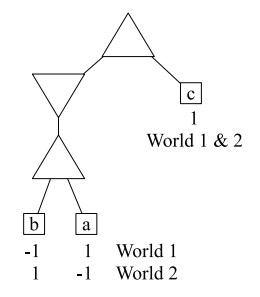
\includegraphics[width = 0.25\linewidth]{strategy-fusion}\label{fig:strategy-fusion}}
   \subfloat[Non-locality]{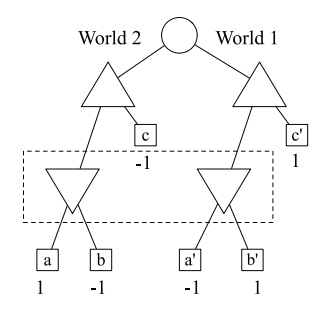
\includegraphics[width = 0.3\linewidth]{non-locality}\label{fig:non-locality}}
   \caption{Diagrams describing two issues of PIMC approach: strategy fusion and non-locality \cite{LonStu2010}.}
   \label{fig:pimc-problems}
\end{figure*}

\subsection{MCTS and PUCT}
\textit{MCTS} (Monte--Carlo Tree Search) is a best-first tree search algorithm consisting of the iterative process of the following three steps: 1) to \textit{select} a leaf node according to a specified selection algorithm, 2) to \textit{evaluate} the leaf node, and 3) to \textit{update} the tree accordingly with the evaluation result.
Then MCTS averages the evaluation results in the subtree rooted at state $s$ to obtain the expected value $V(s)$ of the state. By means of evaluation, Alpha(Go) Zero and this project use neural networks as state value approximators instead of rollout---a totally random search on the tree.
Most selection algorithms are designed to minimise the expected regret of sampling the state $s$ by balancing exploration and exploitation.
Examples of selection algorithms include UCB1 \cite{KocSze2006}, PUCT \cite{Ros2011}, and a variant of PUCT used by AlphaGo, as shown below:
\begin{align*}
   a_t &= \mathop{\operatorname{arg\,max}}\limits_{a} \left( Q(s, a) + U(s, a) \right),
   \\U(s, a) &= c_\textrm{PUCT}\, P(a\mid s)\,\frac{\sqrt{\sum_b N(s, b)}}{1 + N(s, a)}.
\end{align*}
Here $Q(s, a)$ is the value of taking the action $a$ at the state $s$, and $U(s, a)$ is a bonus value to regulate exploration, given by the variant of PUCT. $P(a\mid s)$ is the prior probability of taking the action $a$ at the state $s$, and $N(s, a)$ is the simulation counts of taking $a$ at $s$. $c_\text{PUCT}$ is a constant multiplicative factor to be chosen manually.

The resulting probability distribution $P(a\mid s)$ is proportional to $N(s, a)^{1/\tau}$, where $\tau$ is a hyperparameter deciding how deterministic the choice would be. It is because as $\tau \searrow 0$, $N(s, a)^{1/\tau}$ tends to 0 if $N(s, a) < \max_{b} N(s, b)$.

\subsection{PV-MCTS}
\textit{Policy Value MCTS} (PV-MCTS) uses neural networks to provide a policy $P(a\mid s)$ and a value $V(s)$ for given state $s$. The policy and the value provided by the neural networks are used to estimate the policy and the value of the unvisited leaf node during each step of MCTS. While AlphaGo used two separate networks to approximate $P$ and $V$, AlphaGo Zero used one shared neural network that outputs the prior probabilities and the state value simultaneously.

Experiments from \cite{Sil2017} show that the output policy of PV-MCTS is about 2000 Elo ratings stronger than simply using policy value neural networks to learn the strategy without MCTS.

\subsection{Imperfect Information}
Go-Stop is a game of imperfect (incomplete, or hidden) information. In this section, we introduce the notations used within the report. Let $G$ denotes the set of full states of all possible (Go-Stop) games, and $i\in \{0,1\}$ be the (index of) player. Now, Let $H_i$ denote the set of all hidden states for the player $i$, and $f_i\colon G\to H_i$ be the \textit{observation function} of the player $i$, i.e., $f_i(g)$ is parts of the state of the game $g$ which observable to the player $i$. Note that $f_i$ is surjective, $H_i = f_i(G)$. But usually $f_i$ is not injective, and $f_i^{-1}(f_i(g)) = \{\tilde g\in G\colon f_i(\tilde g) = f_i(g)\}$ denotes the set of game states which are seemingly identical to the player $i$.

\subsection{PIMC}
One popular way of dealing with imperfect information is a method called \textit{Perfect Information Monte--Carlo} (PIMC), also known as \textit{determinization.} With this approach, given a game state with hidden information, a game state of perfect information is sampled in which the current state is chosen from the agent's current information set. For instance, in the game of Rock-Paper-Scissors, the decision of `me' is visible but the decision of opponent is hidden. So PIMC chooses one deterministic game state, where the decision of `me' is the same with the hidden one and the decision of the opponent is one of rock, paper, and scissors. PIMC has shown expert-level performances on games like Bridge \cite{Gin2001} and Skat \cite{Bur2009}, and it has produced strong play on Hearts \cite{Stu2008}.

In 1998, Frank and Basin published an extensive critique of PIMC approach to imperfect information games \cite{FraBas1998}. They suggest two problems residing in the nature of PIMC: strategy fusion and non-locality. In \cref{fig:pimc-problems}, an upward pointing triangle represents a player (\textit{player I}) who wants to maximize the payoff, and a downward pointing triangle represents a player (\textit{player II}) who wants to minimize the payoff.

In \cref{fig:strategy-fusion}, at the first step, the player I has an option to select the right edge, which is always better than selecting the left node. However, by a determinization, even if the player I selects the left edge at the first step, the player I can obtain the payoff 1 no matter which action the player II did, so the player I will be confused between the left edge and the right edge at the first choice. This problem is called \textit{strategy fusion.}

The second error identified is termed \textit{non-locality,} and it is a result of the fact that the value of a node may depend on other regions of the game tree not contained within its subtree, primarily due to the opponent's ability to direct the play towards regions of the tree that they know are favorable for them, using private information. In the game represented by \cref{fig:non-locality}, the best action of player II will be selecting an edge randomly. But, assuming the player I is reasonable, the player II can always know the correct move, because the player I would take the right edge to win the payoff 1 if the player I were in World 1. This means that if there is a chance to play an action for the player II, the game is in World 2, so the player II will take the right edge to take the payoff -1.

Despite those critiques of PIMC, in practice it has often produced strong results in a variety of domains, as indicated by \cite{LonStu2010}.

%%%%%%%%% METHODS
\section{Methods}
\subsection{Self-Play Training Pipeline}
We basically followed the steps of PV-MCTS as described in \cref{sec:background}, but there are miscellaneous differences. First, execute \cref{alg:execute-episode} $n_\text{epi/evol}$ times to gather the training examples. After every call, append the result of it to the replay buffer, and take its recent $n_\text{rep\,buf}$ examples. Split them into minibatches of size $n_\text{mb}$ and train the neural network with those minibatches.

$\mathcal S_g$ is a sample from $f_i^{-1}(f_i(g))$, so PIMC approach is used here. When $\pi_\text{noise}$ is assigned, $\bar e[1]$ represents the average policy produced by MCTS in the game instances in $\mathcal S_g$. By adding a Dirichlet noise $E$, we get an $\pi_\textrm{noise}$, the average policy with a Dirichlet noise. Finally, when an example is appended to $\tilde\ell$, we put $w_\text{reward}\,v + (1 - w_\text{reward})\,\bar q$ as a value for the example. $\bar q$ is the average of expected rewards of the games in $\mathcal S_g$ from the previous neural network, and $v$ is the expected reward from the MCTS simulation. By considering $\bar q$ together, we may reduce the bias from the determinization.

\begin{algorithm}
\small
\setstretch{0.9}
\SetAlgoLined
\SetKwFunction{FMain}{execute\_episode}
   \SetKwProg{Fn}{Function}{:}{}
   \Fn{\FMain{\texttt{NN}}}{
      $\ell \longleftarrow []$; $\tilde\ell \longleftarrow []$;
      $g \longleftarrow \texttt{Game}()$;

      \While{\textbf{not }$g.\texttt{ended}()$}
      {
         $e \longleftarrow []$;

         $i \longleftarrow g.\texttt{current\_player}$;

         $n_\text{hand}\longleftarrow |g.\texttt{hand}(0)| + |g.\texttt{hand}(1)|$;

         $\tau\longleftarrow 1\textbf{ if }n_\textrm{hand} < n_{\tau}\textbf{ else }\tau_{\ll 1}$;

         $\mathcal S_g \longleftarrow \textrm{sample $n_\text{sim\,games}(n_\text{hand})$ games from}$ $f_i^{-1}(f_i(g))$ \text{uniformly at random};

         \ForEach{$\tilde g\in \mathcal S_g$}{
            Call $\texttt{MCTS}(g, \texttt{NN})$ $n_{\text{MCTS/simul}}$ times;

            $a \longleftarrow$ sample an action according to the distribution $\pi(g, \cdot; \tau_{\ll 1})$;

            $e\texttt{.append}((f_i(g), \pi(\tilde g, \cdot; \tau), Q(\tilde g, a), i))$;
         }

         $\bar e\longleftarrow e\texttt{.mean$($axis\,$=0)$}$;

         $\ell\texttt{.append}(\bar e)$;

         $E\sim \operatorname{Dir}(\alpha);\quad \pi_\textrm{noise} \longleftarrow (1-\epsilon)\cdot \bar e[1] + \epsilon \cdot E$;

         $a_\text{next}\longleftarrow$ sample an action according to the distribution $\pi_\textrm{noise}$;

         $g\longleftarrow g\texttt{.next\_state}(a_\text{next})$;
      }

      \ForEach{$(h_i, \pi, \bar q, i)\textbf{ in }\ell$}{
         $v \longleftarrow \texttt{reward}(g, i)$;

         $\tilde\ell\texttt{.append}((h_i, \pi, w_\text{reward}\, v + (1 - w_\text{reward})\, \bar q))$;
      }

      \Return{$\tilde\ell$}
}
\vspace*{1em}
\caption{\texttt{execute\_episode}}
\label{alg:execute-episode}
\end{algorithm}

\subsection{Reward Function}
After a game is terminated, the agent receives a reward measuring how good the agent is doing. In this project, we modeled the reward function considering both scores and whether the agent won:
\begin{align*}
   v(g) =&\, (1\textbf{ if }\text{the agent won}\textbf{ else }-1)
   \\&\cdot (w_\text{win}\cdot 40  + (1-w_\text{win})\,g.\texttt{winners\_score})
\end{align*}
For instance, if $w_\text{win}$ is set to 0.5 and the score for the agent was $-16$, then the reward will be $-(0.5\cdot 40 + 0.5\cdot 16) = -28$.

Note that for the evaluation, we chose $w_\text{win}=0$, that is, $v(g)$ is the raw score from the game.

\subsection{Network Architecture}
While AlphaZero uses a ResNet as a base network architecture, we use a series of fully connected layers as shared network components. Go-Stop board has no geometric properties in it, as opposed to Go, Chess, or Shogi, which AlphaZero deals with. In such games, game pieces placed near to each other and far to each other should be treated differently due to the nature of those games. However, in Go-Stop, everything is either a number or a set of cards having no specific orders. Therefore, it makes no sense to use convolutional layers, where the weights are nonzero only if the row index and the column index are close enough, when we see the convolution operator as a matrix. So we use fully connected layers. The entire network layers are shown below.

\begin{figure}[H]
   \centering
   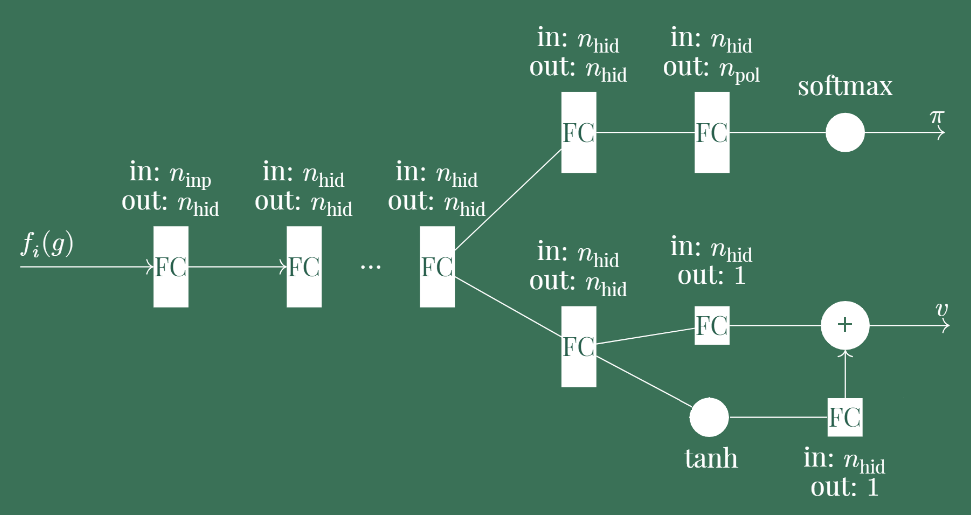
\includegraphics[width = 0.8\linewidth]{network-architecture}
   \label{fig:network-architecture}
   \caption{Network architecture used in the project.}
\end{figure}

\subsection{Optimizer}
The chosen optimizer is a stochastic gradient descent optimizer, with the initial learning rate $10^{-3}$ and the exponential decrease rate $0.96$. The loss function is as follows:
\begin{align*}
   L(\hat p, \hat v; p, v) &= L_\text{policy}(\hat p; p) + L_\text{value}(\hat v; v),\\
   L_\text{policy}(\hat p; p) &= -10\sum_{a} p(a\mid s) \log(\hat p(a\mid s)),\\
   L_\text{value}(\hat v; v) &= (v - \hat v)^2.
\end{align*}
Note that the constant 10 is multiplied in order to equalize the (empirical) magnitudes of two losses.

\subsection{Evaluation}
For both self-play and a match with a random agent, to reduce the fluctuation of results, we use a fixed set of games, in the file \texttt{games.pickle}. However, the fluctuation still exists due to the randomness of the random agent. Further, to limit the effects of luck, for each game, the same game is played just with switching the starting player (refer to \texttt{match\_agents} method.)

\subsection{Implementation Details}

\subsubsection{Encoding Game State}
The encoded game has the following information: my hand, opponent's hand (visible cards only), my and opponent's capture fields, my and opponent's `Go' histories (records the scores of a player when they declared `Go,') the numbers of shakings for me and opponent, my and opponent's stacking histories (who had shaken cards of which month,) my and opponent's scores.

A set of card is encoded to a sum of one-hot vectors representing each element card. For a `Go' history, it is just an array (of maximum length 9) of scores. A stacking history is a sum of one-hot vectors representing months.

\subsubsection{Hyperparameter Choices}
The batch size $B$ is chosen to be 256, which is believed to be in a standard range.

$c_\text{PUCT}=4$, $\epsilon=0.25$, $\alpha=1$, $n_\tau=20$ are chosen as suggested in \cite{Ora2018}.

$n_\text{sim\,games}(t) = \max( \lfloor 2^{(34 - t) / 7}\rfloor, 3)$, $n_\text{MCTS/simul}=50$, $n_{epi/evol} = 35$, $w_\text{reward} = 0.7$ are chosen without any prior knowledge. In particular, first two values are chosen to avoid too-long training process.

As mentioned above, the neural network is trained using $n_\text{rep\,buf}$ most recent examples from the replay buffer. We decided $n_\text{rep\,buf} = 500 + 400c$, where $c$ is the generation count of the network. It is beneficial to phase out early training examples as these contain less valuable information, according to \cite{Ora2018} and \cite{CarOhm2019}.


%%%%%%%%% RESULTS
\section{Results}
\label{sec:results}

\subsection{Quantitative Results}

We tested two network structures, AGS-3 and AGS-6, where the numbers of shared hidden fully connected layers are 3 and 6, \textit{resp.} The loss plots (\cref{fig:loss-plots}) are included.

After the training until 13-th evolutions, AGS-3 showed a performance of gaining $\approx 2$ points on average in the matches with a random agent. And with AGS-6 the average score is $\ge 10$ most of the time in the matches with a random agent. To reproduce it, run \texttt{test\_agents.py} at the root of the backend repository.

\begin{figure}
   \centering
   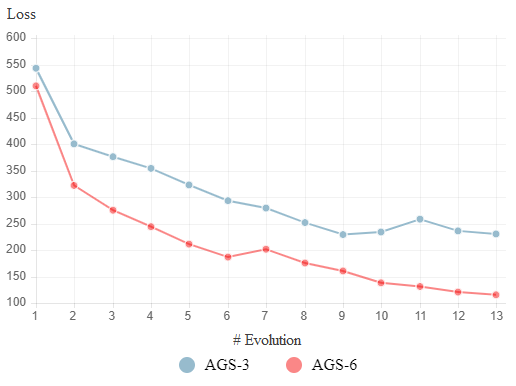
\includegraphics[width=0.8\linewidth]{loss}
   \caption{The loss plots for two networks, AGS-3 and AGS-6.}
   \label{fig:loss-plots}
\end{figure}

We also tried to get Elo ratings of the agents, but the results are too unstable to draw any meaningful conclusion, due to the randomness of the evaluation method.

\subsection{Qualitative Drawbacks}

Both agents seem to be declare `Stop' even when it is fairly able to declare `Go,' as in \cref{fig:drawback-1}. It seems that the MCTS did not provide an enough amount of training examples where it is worthwhile to declare `Go' under that situation.

\begin{figure*}[t]
   \centering
   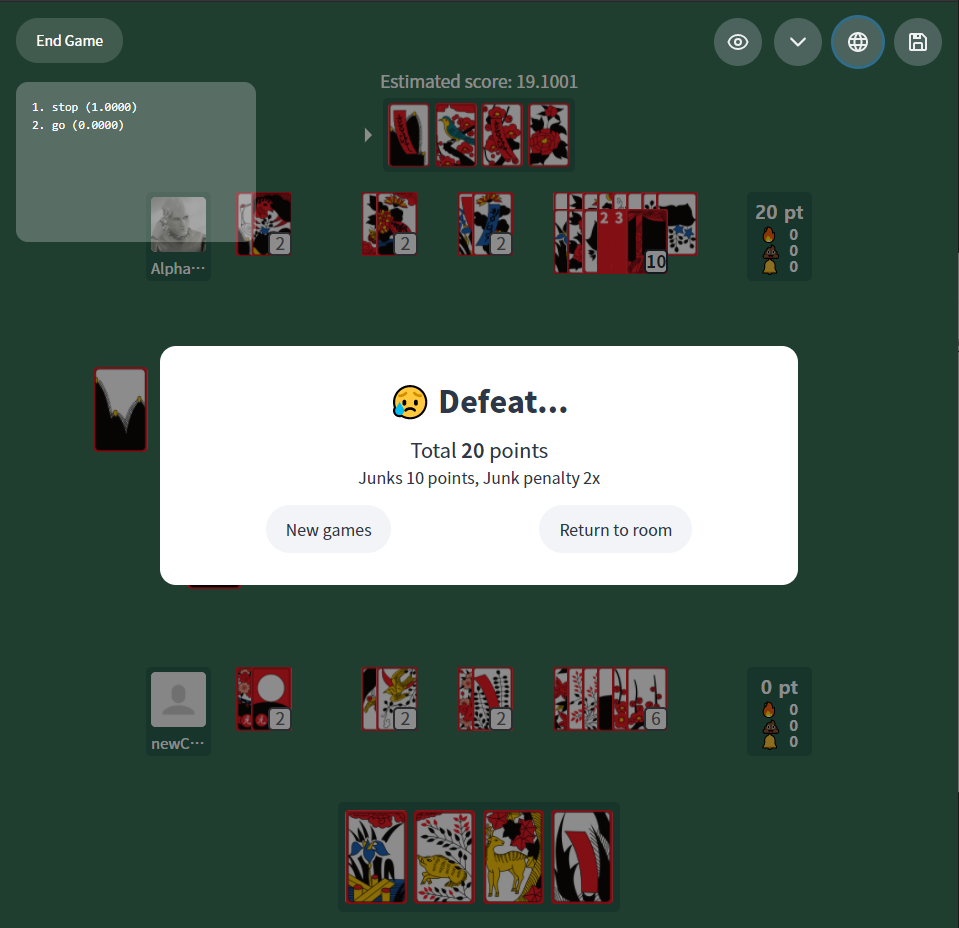
\includegraphics[width=0.48\linewidth]{game-screen-1}
   \hfill
   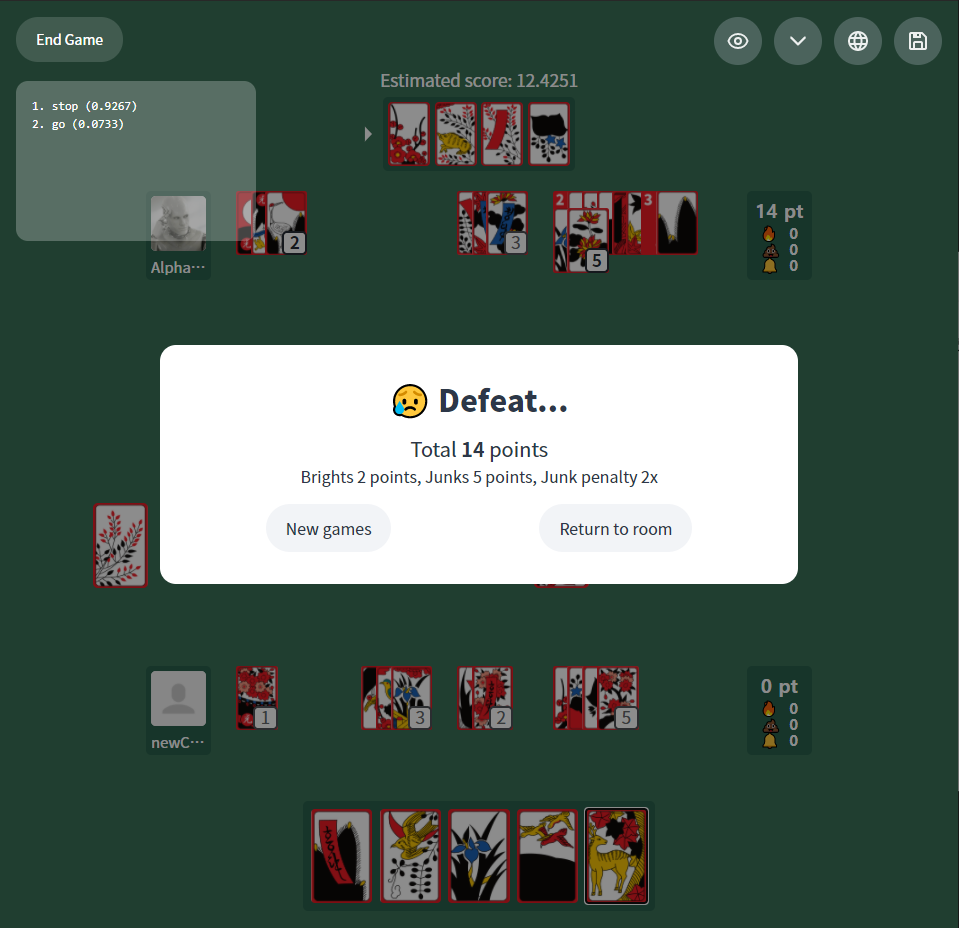
\includegraphics[width=0.48\linewidth]{game-screen-2}
   \caption{The first qualitative drawback. The agent declares `Stop' most of the time. `Go' makes the score multiplied by 2 (when the player had declared 3 or more Go's,) so, declaring `Go' might be better on some occasions.}
   \label{fig:drawback-1}
\end{figure*}

Furthermore, sometimes the agent tries to discard a card even when there are plenty of cards that can be matched, as in \cref{fig:drawback-2}. We guess it is because the agent is aiming for \textit{discard-and-match.}

As predicted in \cref{sec:background}, it seems that both agents also suffer from strategy fusion and non-locality.

\begin{figure}[H]
   \centering
   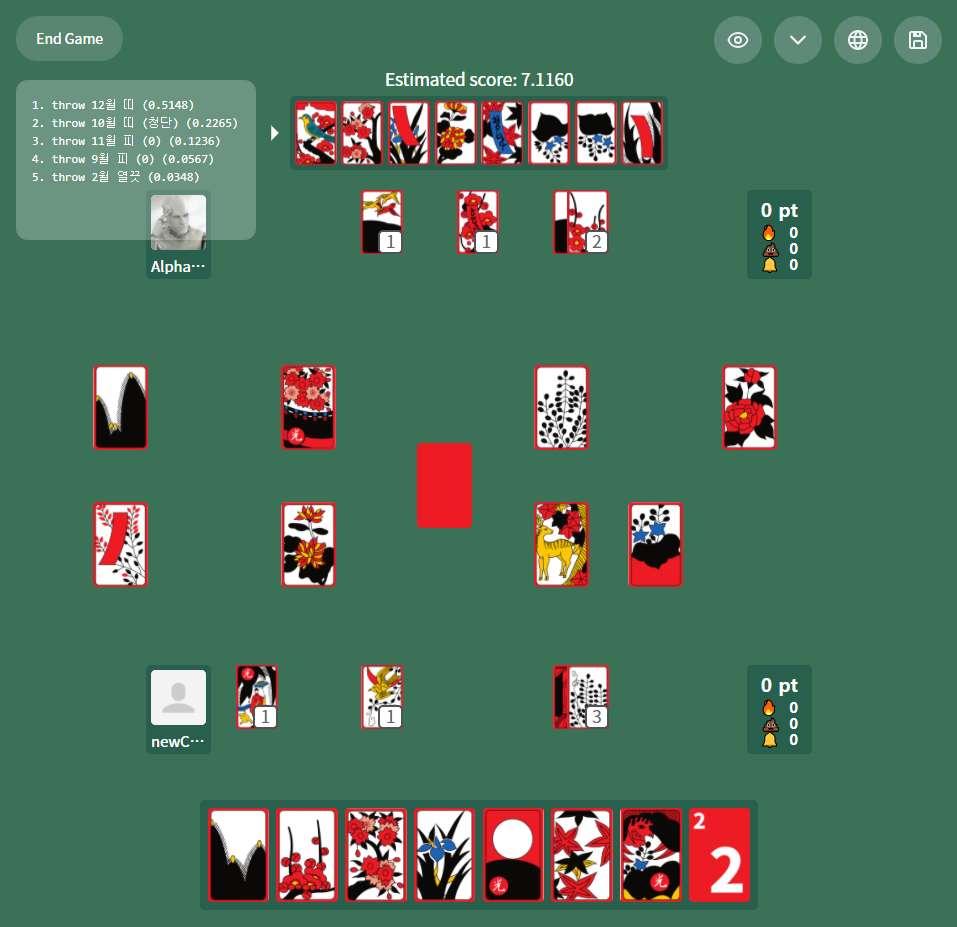
\includegraphics[width=\linewidth]{game-screen-3}
   \caption{The second qualitative drawback. The agent is about to throw a card of December, while there are several cards that can be captured by it, such as the double junk of November, the bright of March, or a junk of September.}
   \label{fig:drawback-2}
\end{figure}


%%%%%%%%% LIMITATIONS
\section{Limitations and Future Works}
\label{sec:limitations}
From the result of \cref{sec:results}, we observed that Go-Stop is quite vulnerable to the negative effects of determinization. This would be because the scores in Go-Stop is changing very rapidly from some stages, and every single action is important where the luck is involved more significantly in it.

Also, we introduced some heuristics (such as considering average of policies of games in $\mathcal S_g$ from the neural network) when we implement PIMC with multiple game instances into Go-Stop, as described in \cref{alg:execute-episode}. It may cause another issue related to the nature of those heuristics, which are not investigated in this project yet.

To resolve those issues, we think the major solution to those is changing the hidden information mechanism from PIMC to another methods, such as ISMCTS \cite{Cow2012}, $\alpha\mu$ search \cite{CazVen2019}, or deep counterfactual value networks \cite{Mor2017} to avoid strategy fusion and non-locality problems.

Also, as the scores in Go-Stop \textit{explode} after `3 Go,' so it would be better if the reward function is being concave on the positive $x$ axis (and \textit{vice versa}), to penalize exponentially growing scores.

Recently, ReBeL \cite{Bro2020} showed a good performance on the game of Poker, and ReBeL is proved to converges to a Nash equilibrium in \textit{any} two players game. If we employ this method, we might obtain a better result.

%%%%%%%%% CONCLUSION
\section{Conclusion}
AlphaZero is a deep reinforcement learning model aiming to solve Go, Chess, or Shogi, which are games of perfect information and having similar geometric structures. By applying the general strategy of AlphaZero to Go-Stop, we obtained an agent getting $\ge 10$-points versus a random agent. There are some drawbacks and inconsistencies found from the agent, as predicted by \cite{FraBas1998}. So, we can conclude that non-randomness and the publicity of information of the game is important to the soundness and convergence of PV-MCTS process used in AlphaZero. To make the agent better, we proposed to use other methods than the naive MCTS to deal with hidden information and to employ other modifications, as written in \cref{sec:limitations}.

\section*{Contributions}
The project proposal is written by Keonwoo Kim, Yongwook Lee, and Junwon Jo. Everything else is implemented by Keonwoo Kim.


\newpage


{\small
\bibliographystyle{ieee_fullname}
\bibliography{main}
}

\end{document}
%
%
%
% CVPR ORIGINAL SAMPLE:
%
%
%

%%%%%%%%% ABSTRACT
\begin{abstract}
   The ABSTRACT is to be in fully-justified italicized text, at the top
   of the left-hand column, below the author and affiliation
   information. Use the word ``Abstract'' as the title, in 12-point
   Times, boldface type, centered relative to the column, initially
   capitalized. The abstract is to be in 10-point, single-spaced type.
   Leave two blank lines after the Abstract, then begin the main text.
   Look at previous CVPR abstracts to get a feel for style and length.
\end{abstract}

%%%%%%%%% BODY TEXT
\section{Introduction}

Please follow the steps outlined below when submitting your manuscript to
the IEEE Computer Society Press.  This style guide now has several
important modifications (for example, you are no longer warned against the
use of sticky tape to attach your artwork to the paper), so all authors
should read this new version.

%-------------------------------------------------------------------------
\subsection{Language}

All manuscripts must be in English.

\subsection{Dual submission}

Please refer to the author guidelines on the CVPR 2020 web page for a
discussion of the policy on dual submissions.

\subsection{Paper length}
Papers, excluding the references section,
must be no longer than eight pages in length. The references section
will not be included in the page count, and there is no limit on the
length of the references section. For example, a paper of eight pages
with two pages of references would have a total length of 10 pages.
{\bf There will be no extra page charges for CVPR 2020.}

Overlength papers will simply not be reviewed.  This includes papers
where the margins and formatting are deemed to have been significantly
altered from those laid down by this style guide.  Note that this
\LaTeX\ guide already sets figure captions and references in a smaller font.
The reason such papers will not be reviewed is that there is no provision for
supervised revisions of manuscripts.  The reviewing process cannot determine
the suitability of the paper for presentation in eight pages if it is
reviewed in eleven.  

%-------------------------------------------------------------------------
\subsection{The ruler}
The \LaTeX\ style defines a printed ruler which should be present in the
version submitted for review.  The ruler is provided in order that
reviewers may comment on particular lines in the paper without
circumlocution.  If you are preparing a document using a non-\LaTeX\
document preparation system, please arrange for an equivalent ruler to
appear on the final output pages.  The presence or absence of the ruler
should not change the appearance of any other content on the page.  The
camera ready copy should not contain a ruler. (\LaTeX\ users may uncomment
the \verb'\cvprfinalcopy' command in the document preamble.)  Reviewers:
note that the ruler measurements do not align well with lines in the paper
--- this turns out to be very difficult to do well when the paper contains
many figures and equations, and, when done, looks ugly.  Just use fractional
references (e.g.\ this line is $095.5$), although in most cases one would
expect that the approximate location will be adequate.

\subsection{Mathematics}

Please number all of your sections and displayed equations.  It is
important for readers to be able to refer to any particular equation.  Just
because you didn't refer to it in the text doesn't mean some future reader
might not need to refer to it.  It is cumbersome to have to use
circumlocutions like ``the equation second from the top of page 3 column
1''.  (Note that the ruler will not be present in the final copy, so is not
an alternative to equation numbers).  All authors will benefit from reading
Mermin's description of how to write mathematics:
\url{http://www.pamitc.org/documents/mermin.pdf}.


\subsection{Blind review}

Many authors misunderstand the concept of anonymizing for blind
review.  Blind review does not mean that one must remove
citations to one's own work---in fact it is often impossible to
review a paper unless the previous citations are known and
available.

Blind review means that you do not use the words ``my'' or ``our''
when citing previous work.  That is all.  (But see below for
techreports.)

Saying ``this builds on the work of Lucy Smith [1]'' does not say
that you are Lucy Smith; it says that you are building on her
work.  If you are Smith and Jones, do not say ``as we show in
[7]'', say ``as Smith and Jones show in [7]'' and at the end of the
paper, include reference 7 as you would any other cited work.

An example of a bad paper just asking to be rejected:
\begin{quote}
\begin{center}
    An analysis of the frobnicatable foo filter.
\end{center}

   In this paper we present a performance analysis of our
   previous paper [1], and show it to be inferior to all
   previously known methods.  Why the previous paper was
   accepted without this analysis is beyond me.

   [1] Removed for blind review
\end{quote}


An example of an acceptable paper:

\begin{quote}
\begin{center}
     An analysis of the frobnicatable foo filter.
\end{center}

   In this paper we present a performance analysis of the
   paper of Smith \etal [1], and show it to be inferior to
   all previously known methods.  Why the previous paper
   was accepted without this analysis is beyond me.

   [1] Smith, L and Jones, C. ``The frobnicatable foo
   filter, a fundamental contribution to human knowledge''.
   Nature 381(12), 1-213.
\end{quote}

If you are making a submission to another conference at the same time,
which covers similar or overlapping material, you may need to refer to that
submission in order to explain the differences, just as you would if you
had previously published related work.  In such cases, include the
anonymized parallel submission~\cite{Authors14} as additional material and
cite it as
\begin{quote}
[1] Authors. ``The frobnicatable foo filter'', F\&G 2014 Submission ID 324,
Supplied as additional material {\tt fg324.pdf}.
\end{quote}

Finally, you may feel you need to tell the reader that more details can be
found elsewhere, and refer them to a technical report.  For conference
submissions, the paper must stand on its own, and not {\em require} the
reviewer to go to a techreport for further details.  Thus, you may say in
the body of the paper ``further details may be found
in~\cite{Authors14b}''.  Then submit the techreport as additional material.
Again, you may not assume the reviewers will read this material.

Sometimes your paper is about a problem which you tested using a tool which
is widely known to be restricted to a single institution.  For example,
let's say it's 1969, you have solved a key problem on the Apollo lander,
and you believe that the CVPR70 audience would like to hear about your
solution.  The work is a development of your celebrated 1968 paper entitled
``Zero-g frobnication: How being the only people in the world with access to
the Apollo lander source code makes us a wow at parties'', by Zeus \etal.

You can handle this paper like any other.  Don't write ``We show how to
improve our previous work [Anonymous, 1968].  This time we tested the
algorithm on a lunar lander [name of lander removed for blind review]''.
That would be silly, and would immediately identify the authors. Instead
write the following:
\begin{quotation}
\noindent
   We describe a system for zero-g frobnication.  This
   system is new because it handles the following cases:
   A, B.  Previous systems [Zeus et al. 1968] didn't
   handle case B properly.  Ours handles it by including
   a foo term in the bar integral.

   ...

   The proposed system was integrated with the Apollo
   lunar lander, and went all the way to the moon, don't
   you know.  It displayed the following behaviours
   which show how well we solved cases A and B: ...
\end{quotation}
As you can see, the above text follows standard scientific convention,
reads better than the first version, and does not explicitly name you as
the authors.  A reviewer might think it likely that the new paper was
written by Zeus \etal, but cannot make any decision based on that guess.
He or she would have to be sure that no other authors could have been
contracted to solve problem B.
\medskip

\noindent
FAQ\medskip\\
{\bf Q:} Are acknowledgements OK?\\
{\bf A:} No.  Leave them for the final copy.\medskip\\
{\bf Q:} How do I cite my results reported in open challenges?
{\bf A:} To conform with the double blind review policy, you can report results of other challenge participants together with your results in your paper. For your results, however, you should not identify yourself and should not mention your participation in the challenge. Instead present your results referring to the method proposed in your paper and draw conclusions based on the experimental comparison to other results.\medskip\\



\begin{figure}[t]
\begin{center}
\fbox{\rule{0pt}{2in} \rule{0.9\linewidth}{0pt}}
   %\includegraphics[width=0.8\linewidth]{egfigure.eps}
\end{center}
   \caption{Example of caption.  It is set in Roman so that mathematics
   (always set in Roman: $B \sin A = A \sin B$) may be included without an
   ugly clash.}
\label{fig:long}
\label{fig:onecol}
\end{figure}

\subsection{Miscellaneous}

\noindent
Compare the following:\\
\begin{tabular}{ll}
 \verb'$conf_a$' &  $conf_a$ \\
 \verb'$\mathit{conf}_a$' & $\mathit{conf}_a$
\end{tabular}\\
See The \TeX book, p165.

The space after \eg, meaning ``for example'', should not be a
sentence-ending space. So \eg is correct, {\em e.g.} is not.  The provided
\verb'\eg' macro takes care of this.

When citing a multi-author paper, you may save space by using ``et alia'',
shortened to ``\etal'' (not ``{\em et.\ al.}'' as ``{\em et}'' is a complete word.)
However, use it only when there are three or more authors.  Thus, the
following is correct: ``
   Frobnication has been trendy lately.
   It was introduced by Alpher~\cite{Alpher02}, and subsequently developed by
   Alpher and Fotheringham-Smythe~\cite{Alpher03}, and Alpher \etal~\cite{Alpher04}.''

This is incorrect: ``... subsequently developed by Alpher \etal~\cite{Alpher03} ...''
because reference~\cite{Alpher03} has just two authors.  If you use the
\verb'\etal' macro provided, then you need not worry about double periods
when used at the end of a sentence as in Alpher \etal.

For this citation style, keep multiple citations in numerical (not
chronological) order, so prefer \cite{Alpher03,Alpher02,Authors14} to
\cite{Alpher02,Alpher03,Authors14}.


\begin{figure*}
\begin{center}
\fbox{\rule{0pt}{2in} \rule{.9\linewidth}{0pt}}
\end{center}
   \caption{Example of a short caption, which should be centered.}
\label{fig:short}
\end{figure*}

%------------------------------------------------------------------------
\section{Formatting your paper}

All text must be in a two-column format. The total allowable width of the
text area is $6\frac78$ inches (17.5 cm) wide by $8\frac78$ inches (22.54
cm) high. Columns are to be $3\frac14$ inches (8.25 cm) wide, with a
$\frac{5}{16}$ inch (0.8 cm) space between them. The main title (on the
first page) should begin 1.0 inch (2.54 cm) from the top edge of the
page. The second and following pages should begin 1.0 inch (2.54 cm) from
the top edge. On all pages, the bottom margin should be 1-1/8 inches (2.86
cm) from the bottom edge of the page for $8.5 \times 11$-inch paper; for A4
paper, approximately 1-5/8 inches (4.13 cm) from the bottom edge of the
page.

%-------------------------------------------------------------------------
\subsection{Margins and page numbering}

All printed material, including text, illustrations, and charts, must be kept
within a print area 6-7/8 inches (17.5 cm) wide by 8-7/8 inches (22.54 cm)
high.
Page numbers should be in footer with page numbers, centered and .75
inches from the bottom of the page and make it start at the correct page
number rather than the 4321 in the example.  To do this fine the line (around
line 23)
\begin{verbatim}
%\ifcvprfinal\pagestyle{empty}\fi
\setcounter{page}{4321}
\end{verbatim}
where the number 4321 is your assigned starting page.

Make sure the first page is numbered by commenting out the first page being
empty on line 46
\begin{verbatim}
%\thispagestyle{empty}
\end{verbatim}


%-------------------------------------------------------------------------
\subsection{Type-style and fonts}

Wherever Times is specified, Times Roman may also be used. If neither is
available on your word processor, please use the font closest in
appearance to Times to which you have access.

MAIN TITLE. Center the title 1-3/8 inches (3.49 cm) from the top edge of
the first page. The title should be in Times 14-point, boldface type.
Capitalize the first letter of nouns, pronouns, verbs, adjectives, and
adverbs; do not capitalize articles, coordinate conjunctions, or
prepositions (unless the title begins with such a word). Leave two blank
lines after the title.

AUTHOR NAME(s) and AFFILIATION(s) are to be centered beneath the title
and printed in Times 12-point, non-boldface type. This information is to
be followed by two blank lines.

The ABSTRACT and MAIN TEXT are to be in a two-column format.

MAIN TEXT. Type main text in 10-point Times, single-spaced. Do NOT use
double-spacing. All paragraphs should be indented 1 pica (approx. 1/6
inch or 0.422 cm). Make sure your text is fully justified---that is,
flush left and flush right. Please do not place any additional blank
lines between paragraphs.

Figure and table captions should be 9-point Roman type as in
Figures~\ref{fig:onecol} and~\ref{fig:short}.  Short captions should be centred.

\noindent Callouts should be 9-point Helvetica, non-boldface type.
Initially capitalize only the first word of section titles and first-,
second-, and third-order headings.

FIRST-ORDER HEADINGS. (For example, {\large \bf 1. Introduction})
should be Times 12-point boldface, initially capitalized, flush left,
with one blank line before, and one blank line after.

SECOND-ORDER HEADINGS. (For example, { \bf 1.1. Database elements})
should be Times 11-point boldface, initially capitalized, flush left,
with one blank line before, and one after. If you require a third-order
heading (we discourage it), use 10-point Times, boldface, initially
capitalized, flush left, preceded by one blank line, followed by a period
and your text on the same line.

%-------------------------------------------------------------------------
\subsection{Footnotes}

Please use footnotes\footnote {This is what a footnote looks like.  It
often distracts the reader from the main flow of the argument.} sparingly.
Indeed, try to avoid footnotes altogether and include necessary peripheral
observations in
the text (within parentheses, if you prefer, as in this sentence).  If you
wish to use a footnote, place it at the bottom of the column on the page on
which it is referenced. Use Times 8-point type, single-spaced.


%-------------------------------------------------------------------------
\subsection{References}

List and number all bibliographical references in 9-point Times,
single-spaced, at the end of your paper. When referenced in the text,
enclose the citation number in square brackets, for
example~\cite{Authors14}.  Where appropriate, include the name(s) of
editors of referenced books.

\begin{table}
\begin{center}
\begin{tabular}{|l|c|}
\hline
Method & Frobnability \\
\hline\hline
Theirs & Frumpy \\
Yours & Frobbly \\
Ours & Makes one's heart Frob\\
\hline
\end{tabular}
\end{center}
\caption{Results.   Ours is better.}
\end{table}

%-------------------------------------------------------------------------
\subsection{Illustrations, graphs, and photographs}

All graphics should be centered.  Please ensure that any point you wish to
make is resolvable in a printed copy of the paper.  Resize fonts in figures
to match the font in the body text, and choose line widths which render
effectively in print.  Many readers (and reviewers), even of an electronic
copy, will choose to print your paper in order to read it.  You cannot
insist that they do otherwise, and therefore must not assume that they can
zoom in to see tiny details on a graphic.

When placing figures in \LaTeX, it's almost always best to use
\verb+\includegraphics+, and to specify the  figure width as a multiple of
the line width as in the example below
{\small\begin{verbatim}
   \usepackage[dvips]{graphicx} ...
   \includegraphics[width=0.8\linewidth]
                   {myfile.eps}
\end{verbatim}
}


%-------------------------------------------------------------------------
\subsection{Color}

Please refer to the author guidelines on the CVPR 2020 web page for a discussion
of the use of color in your document.

%------------------------------------------------------------------------
\section{Final copy}

You must include your signed IEEE copyright release form when you submit
your finished paper. We MUST have this form before your paper can be
published in the proceedings.

Please direct any questions to the production editor in charge of these 
proceedings at the IEEE Computer Society Press: 
\url{https://www.computer.org/about/contact}. 
